\section{Programming Model}
\label{sec:model}

\begin{figure}
\begin{center}
  \begin{ocaml}
  module type CANVAS = sig
    type pixel = {r:char; g:char; b:char}
    type tree =
      | N of pixel
      | B of {tl: tree; tr: tree; bl: tree; br: tree}
    type t = {max_x:int; max_y:int; canvas:tree}
    type loc = {x:int; y:int}

    val new_canvas: int -> int -> t
    val set_px: t -> loc -> pixel -> t
    val get_px: t -> loc -> pixel
    val merge: (* lca *)t -> (* v1 *)t -> (* v2 *)t -> t
  end
  \end{ocaml}
\end{center}
\caption{\drawsome: a sample \name application}
\label{fig:canvas-sig}
\end{figure}

In this section, we describe the \name programming model through the
example of a collaborative drawing application we call \drawsome.
Fig.~\ref{fig:canvas-sig} shows the signature of the \drawsome
application. \drawsome represents a free-hand drawing canvas in terms
of a tree of quadrants.  Each quadrant is simply a leaf node
containing a single pixel (\C{r},\C{g}, or \C{b}) or a tree, if the
quadrant contains multiple pixels of different colors. Quadrants are
\begin{wrapfigure}{l}{.4\textwidth}
\centering
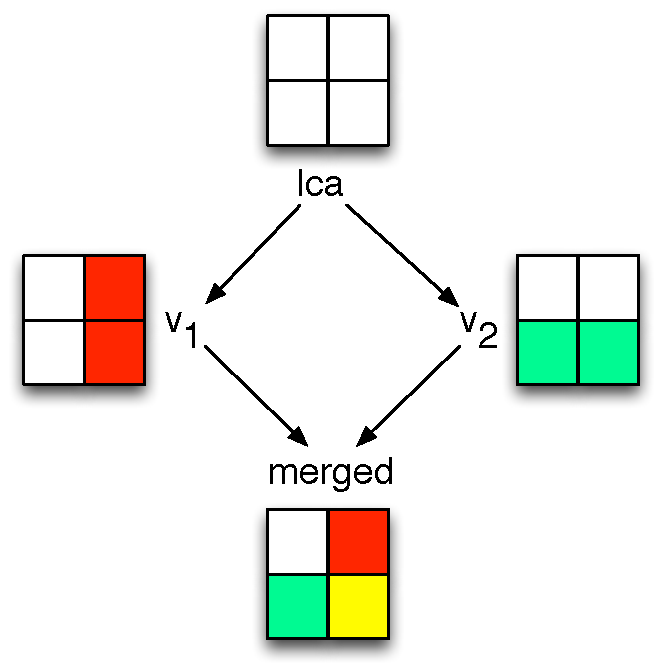
\includegraphics[scale=0.43]{Figures/canvas-merging}
\caption{Merging concurrent versions (\C{v1} and \C{v2}) of a drawing
canvas. \C{lca} is their common ancestor.}
\label{fig:canvas-merging}
\end{wrapfigure}
expanded into a tree structures as and when pixels are colored.  The
representation is thus optimized for sparse canvases, such as
whiteboards. The application supports three simple operations:
creating a new canvas, setting the pixel at a specified coordinate,
and returning the pixel at a given coordinate. The \C{merge} function
is explained below.  \drawsome lets multiple users collaborate on a
canvas that is conceptually shared among them. Under a shared-memory
abstraction, there would be a single copy of the canvas that is
updated concurrently by multiple clients; from the perspective of any
single client, the canvas could change without any explicit
intervention. \name ascribes functional semantics to sharing by
letting each client work on its own version of the state (the tree
data structure in this example), later merging concurrent versions
on-demand.  Thus, the primary artifact of the \name programming model
is a versioned data structure in which different versions are managed
by different clients.

%% The library operates on a representation of versioned data
%% structures optimized for persistence on disk
%% (Sec.~\ref{sec:persistence}).  \name's meta-programming component
%% automatically synthesizes this representation, along with the
%% functions that translate between representations, for the data type
%% definitions marked with the ppx~\cite{ppx} directive \C{deriving
%%   versioned}. Concretely, for the \C{Canvas} module, \name synthesizes
%% a \C{Canvas.Versioned} module with a type \C{t}, and functions
%% \C{of\_canvas} and \C{to\_canvas} of types \C{Canvas.t $\rightarrow$
%%   t} and \C{t $\rightarrow$ Canvas.t}, respectively.

\name requires a three-way \C{merge} function to merge concurrent
versions of a drawing canvas (see Fig.~\ref{fig:merge-canvas}) that
includes includes two concurrent versions (\C{v1} and \C{v2}),
and their lowest common ancestor (\C{lca}) - the version from which the
two concurrent versions evolved independently. The merge function can
make use of the pixel values of the common ancestor to merge the pixel
values on both the canvases. For instance, if the color of a pixel in
\C{v1} is white, and in \C{v2} it is green, and its color in \C{lca}
is white, then it means that only \C{v2} modified the color. Hence the
pixel is colored green in the merged canvas. On the other hand, if the
pixel is red in \C{v1}, then it means that both \C{v1} and \C{v2} have
modified the color. In such case, an appropriate color-mixing algorithm
can be used to determine the color of pixel.  For instance, the pixel
can be colored yellow - an additive combination of red and green. The
logic is illustrated in Fig.~\ref{fig:canvas-merging}.
\begin{figure}
\begin{center}
  \begin{ocaml}
let color_mix px1 px2 : pixel =
let f = Char.code in
let h x y = Char.chr @@ (x + y)/ 2 in
let (r1,g1,b1) = (f px1.r, f px1.g, f px1.b) in
let (r2,g2,b2) = (f px2.r, f px2.g, f px2.b) in
let (r,g,b) = (h r1 r2, h g1 g2, h b1 b2) in {r=r; g=g; b=b}

let b_of_n px = B {tl_t=N px; tr_t=N px; bl_t=N px; br_t=N px}

let rec merge lca v1 v2 =
  if v1=v2 then v1
  else if v1=lca then v2
  else if v2=lca then v1
  else match (lca,v1,v2) with
    | (_, B _, N px2) -> merge lca v1 @@ b_of_n px2
    | (_, N px1, B _) -> merge lca (b_of_n px1) v2
    | (N px, B _, B _) -> merge (b_of_n px) v1 v2
    | (B x, B x1, B x2) ->
        let tl_t' = merge x.tl_t x1.tl_t x2.tl_t in
        let tr_t' = merge x.tr_t x1.tr_t x2.tr_t in
        let bl_t' = merge x.bl_t x1.bl_t x2.bl_t in
        let br_t' = merge x.br_t x1.br_t x2.br_t in
          B {tl_t=tl_t'; tr_t=tr_t'; bl_t=bl_t'; br_t=br_t'}
    | (_, N px1, N px2) ->
        (* pixels are merged by mixing colors *)
        let px' = color_mix px1 px2 in N px'
 \end{ocaml}
\caption{Merging different versions of a canvas.}
\label{fig:merge-canvas}
\end{center}
\end{figure}

\name\ lets programmers define and compose concurrent computations
around versioned data structures.  Fig.~\ref{fig:dali-monad} shows the
signature of the \nameMonad module that implements the programming
model along the lines of the well-known \C{State} monad. The monad
encapsulates a versioned functional state (\C{'a}) and the type
\C{('a, 'b) t} represents a monadic computation that returns a \C{'b}
result.  Functions \C{return} and \C{bind} have their usual monadic
\begin{figure}
\begin{center}
  \begin{ocaml}
  module type VML = sig
    type ('a, 'b) t
    val return : 'b -> ('a, 'b) t
    val bind : ('a, 'b) t -> ('b -> ('a, 'c) t) -> ('a, 'c) t
    val get_current_version: unit -> ('a, 'a) t
    val with_init_version_do: 'a -> ('a, 'b) t -> 'b
    val fork_version : ('a, 'b) t -> ('a, unit) t
    val sync_next_version: unit -> 'a -> ('a, 'a) t
  end
  \end{ocaml}
  \caption{Signature of the \name monad}
  \label{fig:dali-monad}
\end{center}
\end{figure}
interpretation. \C{get\_current\_version} is like the \C{State}
monad's \C{get}; it returns the versioned state encapsulated by the
monad. To initiate a computation, we use \C{with\_init\_version\_do}
which runs a monadic computation against a given initial version and
returns the result. The \C{fork\_version} operation returns a
computation that forks a new concurrent version from the current
version, and runs the given monadic computation asynchronously against
the forked version.  \C{sync\_next\_version} (simply called \C{sync})
accepts a \emph{proposal} for the next version of the state; this
proposal is the current local version of the state that reflects local
modifications not yet witnessed by any other concurrently executing
computation.  The operation returns (via a monad) the actual next
version, which becomes the current version for the rest of the
computation.  This version is created by merging the proposal with a
subset of concurrent versions that have become available since the
last merge or fork. Thus, \C{sync} effectively lets a computation
synchronize with a subset of concurrent computations to obtain their
latest updates.

\begin{figure}
\centering
\begin{tabular}{l||l||l}
\begin{ocaml}
let alice_f : C.t unit t =
  get () >>= fun c0 ->
  fork bob_f >>= fun () ->
  let c0' = C.draw_line c0
    {x=0;y=0}
    {x=4;y=0} in
  sync () ~v:c0' >>=
  fun c1 ->
  let c1' = C.draw_line c1
    {x=0;y=4}
    {x=4;y=4} in
  sync () ~v:c1' >>=
  fun c2 -> return ()
\end{ocaml}
&
\begin{ocaml}
let bob_f : C.t unit t =
  get () >>= fun c0 ->
  fork cheryl_f >>=
  fun () ->
  let c0' = C.draw_line c0
    {x=0;y=0}
    {x=0;y=4} in
  sync () ~v:c0' >>=
  fun c1 -> sync () >>=
  fun c2 -> return ()
\end{ocaml}
&
\begin{ocaml}
let cheryl_f : C.t unit t =
  get () >>= fun c0 ->
  let c0' = C.draw_line c0
    {x=4;y=0}
    {x=4;y=0} in
  sync () ~v:c0' >>=
  fun c1 -> sync () >>=
  fun c2 -> return ()
\end{ocaml}
\\
\end{tabular}
\caption{\drawsome: A collaborative drawing session between Alice,
Bob, and Cheryl}
\label{fig:canvas-sessions-code}
\end{figure}

Fig.~\ref{fig:canvas-sessions-code} demonstrates how a collaborative
drawing session between Alice, Bob and Cheryl can be composed using
\name. A possible execution of the session is visualized in
Fig.~\ref{fig:canvas-sessions}. Assume that the session starts with
Alice on a $5\times 5$ blank canvas, as shown below:
\begin{ocaml}
  module C = Canvas;;
  with_init_version_do (C.new_blank 5 5) alice_f
\end{ocaml}
Alice starts by reading the current version of the canvas, which is
blank. She then invites Bob for collaboration by forking a new
concurrent version for Bob. Bob, in turn, invites Cheryl for
\begin{figure}
\centering
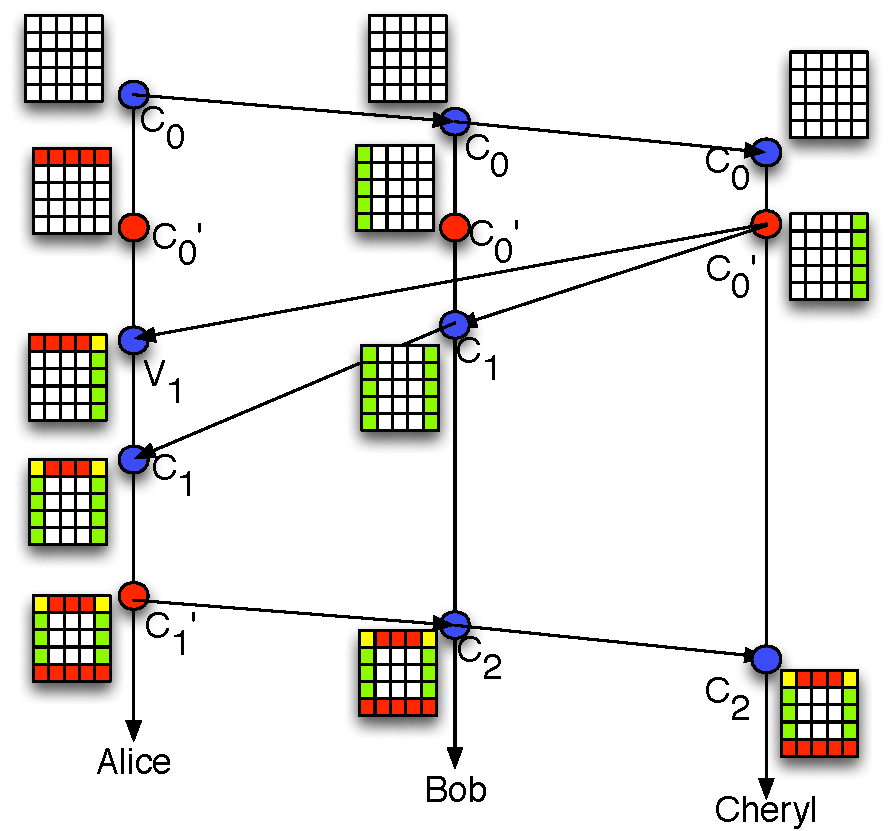
\includegraphics[scale=0.6]{Figures/canvas-sessions}
\caption{\drawsome: Collaborative drawing session visualized}
\label{fig:canvas-sessions}
\end{figure}
collaboration. All three of them start working on the blank canvas.
Alice draws a red horizontal line from $(0,0)$ (top-left) to $(4,0)$
(top-right) using \C{C.draw\_line}.\footnote{Its definition is not
  shown, but can be constructed using \C{set\_px}.} Meanwhile, Bob
draws a green vertical line from $(0,0)$ to $(0,4)$, and Cheryl draws
a similar line from $(4,0)$ to $(4,4)$. All three of them call
\C{sync} with their respective proposals ($C_0'$). While any partial
ordering of concurrent \C{syncs} is valid, we consider a linear order
where Cheryl's \C{sync} happens first, followed by Bob's and then
Alice's.  Cheryl's \C{sync} does not find any concurrent versions,
hence installs the proposed version ($C_0'$) as the next version on
Cheryl's branch. Bob's \C{sync} finds Cheryl's $C_0'$ as a concurrent
version, and merges it with its proposal to produce the next version
$C_1$, which is then installed on Bob's branch.  The lowest common
ancestor (LCA) for this merge is the initial version ($C_0$), and the
two concurrent versions are Bob's $C_0'$ and Cheryl's $C_0'$. Next,
Alice's \C{sync} finds Cheryl's $C_0'$ and Bob's $C_1$ as concurrent
versions, and merges them successively with Alice's proposal. For the
first merge, the two concurrent versions are Alice's $C_0'$ and
Cheryl's $C_0'$, and the LCA is the initial version ($C_0$). The
result of this merge is installed as the next version ($\C{V_1}$) on
Alice's branch. For the next merge, the two concurrent versions are
Alice's $V_1$ and Bob's $C_1$ and the LCA is Cheryl's
$C_0'$\footnote{Thus, the LCA of versions on two branches can lie
  outside both the branches.}. The result ($C_1$) becomes the next
version on Alice's branch, and the return value of Alice's \C{sync}.
Next, Alice draws a red horizontal line from $(0,4)$ to $(4,4)$,
proposes this canvas (\C{c1'} in the first column of
Fig.~\ref{fig:canvas-sessions-code}) as the next version to \C{sync}.
Since there are no concurrent versions, $C_1'$ becomes her next
version. The subsequent \C{sync} operations from Bob and Cheryl
propose no new versions, hence simply obtain Alice's $C_1'$ as next
versions.
